\documentclass[twoside]{book}

% Packages required by doxygen
\usepackage{fixltx2e}
\usepackage{calc}
\usepackage{doxygen}
\usepackage[export]{adjustbox} % also loads graphicx
\usepackage{graphicx}
\usepackage[utf8]{inputenc}
\usepackage{makeidx}
\usepackage{multicol}
\usepackage{multirow}
\PassOptionsToPackage{warn}{textcomp}
\usepackage{textcomp}
\usepackage[nointegrals]{wasysym}
\usepackage[table]{xcolor}

% Font selection
\usepackage[T1]{fontenc}
\usepackage[scaled=.90]{helvet}
\usepackage{courier}
\usepackage{amssymb}
\usepackage{sectsty}
\renewcommand{\familydefault}{\sfdefault}
\allsectionsfont{%
  \fontseries{bc}\selectfont%
  \color{darkgray}%
}
\renewcommand{\DoxyLabelFont}{%
  \fontseries{bc}\selectfont%
  \color{darkgray}%
}
\newcommand{\+}{\discretionary{\mbox{\scriptsize$\hookleftarrow$}}{}{}}

% Page & text layout
\usepackage{geometry}
\geometry{%
  a4paper,%
  top=2.5cm,%
  bottom=2.5cm,%
  left=2.5cm,%
  right=2.5cm%
}
\tolerance=750
\hfuzz=15pt
\hbadness=750
\setlength{\emergencystretch}{15pt}
\setlength{\parindent}{0cm}
\setlength{\parskip}{3ex plus 2ex minus 2ex}
\makeatletter
\renewcommand{\paragraph}{%
  \@startsection{paragraph}{4}{0ex}{-1.0ex}{1.0ex}{%
    \normalfont\normalsize\bfseries\SS@parafont%
  }%
}
\renewcommand{\subparagraph}{%
  \@startsection{subparagraph}{5}{0ex}{-1.0ex}{1.0ex}{%
    \normalfont\normalsize\bfseries\SS@subparafont%
  }%
}
\makeatother

% Headers & footers
\usepackage{fancyhdr}
\pagestyle{fancyplain}
\fancyhead[LE]{\fancyplain{}{\bfseries\thepage}}
\fancyhead[CE]{\fancyplain{}{}}
\fancyhead[RE]{\fancyplain{}{\bfseries\leftmark}}
\fancyhead[LO]{\fancyplain{}{\bfseries\rightmark}}
\fancyhead[CO]{\fancyplain{}{}}
\fancyhead[RO]{\fancyplain{}{\bfseries\thepage}}
\fancyfoot[LE]{\fancyplain{}{}}
\fancyfoot[CE]{\fancyplain{}{}}
\fancyfoot[RE]{\fancyplain{}{\bfseries\scriptsize Generated by Doxygen }}
\fancyfoot[LO]{\fancyplain{}{\bfseries\scriptsize Generated by Doxygen }}
\fancyfoot[CO]{\fancyplain{}{}}
\fancyfoot[RO]{\fancyplain{}{}}
\renewcommand{\footrulewidth}{0.4pt}
\renewcommand{\chaptermark}[1]{%
  \markboth{#1}{}%
}
\renewcommand{\sectionmark}[1]{%
  \markright{\thesection\ #1}%
}

% Indices & bibliography
\usepackage{natbib}
\usepackage[titles]{tocloft}
\setcounter{tocdepth}{3}
\setcounter{secnumdepth}{5}
\makeindex

% Hyperlinks (required, but should be loaded last)
\usepackage{ifpdf}
\ifpdf
  \usepackage[pdftex,pagebackref=true]{hyperref}
\else
  \usepackage[ps2pdf,pagebackref=true]{hyperref}
\fi
\hypersetup{%
  colorlinks=true,%
  linkcolor=blue,%
  citecolor=blue,%
  unicode%
}

% Custom commands
\newcommand{\clearemptydoublepage}{%
  \newpage{\pagestyle{empty}\cleardoublepage}%
}

\usepackage{caption}
\captionsetup{labelsep=space,justification=centering,font={bf},singlelinecheck=off,skip=4pt,position=top}

%===== C O N T E N T S =====

\begin{document}

% Titlepage & ToC
\hypersetup{pageanchor=false,
             bookmarksnumbered=true,
             pdfencoding=unicode
            }
\pagenumbering{roman}
\begin{titlepage}
\vspace*{7cm}
\begin{center}%
{\Large G\+R\+E\+M\+L\+I\+NS \\[1ex]\large 1.\+0 }\\
\vspace*{1cm}
{\large Generated by Doxygen 1.8.11}\\
\end{center}
\end{titlepage}
\clearemptydoublepage
\tableofcontents
\clearemptydoublepage
\pagenumbering{arabic}
\hypersetup{pageanchor=true}

%--- Begin generated contents ---
\chapter{G\+R\+E\+M\+L\+I\+NS}
\label{md_README}
\hypertarget{md_README}{}
G\+R\+E\+M\+L\+I\+NS -\/ Ge\+R\+Enciador de Memória com L\+Ista e\+Ncadeada Simples (Memory Manager with Simple Linked List)

\subsection*{Authors}

The project were developed using Cloud9 I\+DE by\+:

Johnnylee Bryan Marques da Rocha -\/ \href{https://github.com/kfjohnny2}{\tt Git\+Hub}

Pedro Arthur Medeiros Fernandes -\/ \href{https://github.com/pedroarthur-mf}{\tt Git\+Hub}

\subsection*{About}

Is a memory requirement system that will take reserved block of memory and do some manipulations. Small blocks can be created by client to allocate inside the bigger block.

\subsection*{Functionality}

There is a class called \char`\"{}\+S\+L\+Pool\char`\"{} for the implementation of the methods from the abstract class \char`\"{}\+Storage\+Pool\char`\"{}.

\subsubsection*{These methods are\+:}


\begin{DoxyCode}
\textcolor{keywordtype}{void} *Allocate ( std::size\_t ); \textcolor{comment}{// Used to insert some bytes of memory inside the bigger block;}

\textcolor{keywordtype}{void} *Best\_Allocate ( std::size\_t ); \textcolor{comment}{// Used to insert some bytes seeking for the nearest empty block for
       best time improvement;}

\textcolor{keywordtype}{void} Free( \textcolor{keywordtype}{void} * ); \textcolor{comment}{// Used to liberate required bytes of memory from the bigger block;}
\end{DoxyCode}


\subsection*{How to Compile}

There a two types of test, the timing test. The first\+: will use the method Storage\+Pool\+Test, that test the alocation of memory using the \hyperlink{class_storage_pool}{Storage\+Pool} and calculating the time of the \hyperlink{class_event}{Event}. The S\+O\+Memory\+Test calculate the time based on the SO timing
\begin{DoxyItemize}
\item For this test type the following command on terminal inside de \char`\"{}\+G\+R\+E\+M\+L\+I\+N\+S\char`\"{} folder\+: 
\begin{DoxyCode}
1 g++ -Wall -std=c++11 -I include/ src/drive\_gremlins.cpp -o bin/gremlins
2 
3 ./bin/gremlins
\end{DoxyCode}

\end{DoxyItemize}

The second\+: Will make a series of manipulations using normal Allocate, Best-\/\+Fit Allocate and Free and printing the memory block state in each operation.
\begin{DoxyItemize}
\item Following the same instruction above, type\+: 
\begin{DoxyCode}
1 g++ -Wall -std=c++11 -I include/ src/drive\_gremlins2.cpp -o bin/gremlins
2 
3 ./bin/gremlins
\end{DoxyCode}
 
\end{DoxyItemize}
\chapter{Hierarchical Index}
\section{Class Hierarchy}
This inheritance list is sorted roughly, but not completely, alphabetically\+:\begin{DoxyCompactList}
\item \contentsline{section}{Event}{\pageref{class_event}}{}
\item \contentsline{section}{S\+L\+Pool\+:\+:Header}{\pageref{struct_s_l_pool_1_1_header}}{}
\begin{DoxyCompactList}
\item \contentsline{section}{S\+L\+Pool\+:\+:Block}{\pageref{struct_s_l_pool_1_1_block}}{}
\end{DoxyCompactList}
\item \contentsline{section}{Storage\+Pool}{\pageref{class_storage_pool}}{}
\begin{DoxyCompactList}
\item \contentsline{section}{S\+L\+Pool}{\pageref{class_s_l_pool}}{}
\end{DoxyCompactList}
\item \contentsline{section}{Tag}{\pageref{struct_tag}}{}
\end{DoxyCompactList}

\chapter{Class Index}
\section{Class List}
Here are the classes, structs, unions and interfaces with brief descriptions\+:\begin{DoxyCompactList}
\item\contentsline{section}{\hyperlink{struct_s_l_pool_1_1_block}{S\+L\+Pool\+::\+Block} }{\pageref{struct_s_l_pool_1_1_block}}{}
\item\contentsline{section}{\hyperlink{class_event}{Event} \\*A class that creates a pair address/time-\/stamp }{\pageref{class_event}}{}
\item\contentsline{section}{\hyperlink{struct_s_l_pool_1_1_header}{S\+L\+Pool\+::\+Header} }{\pageref{struct_s_l_pool_1_1_header}}{}
\item\contentsline{section}{\hyperlink{class_s_l_pool}{S\+L\+Pool} }{\pageref{class_s_l_pool}}{}
\item\contentsline{section}{\hyperlink{class_storage_pool}{Storage\+Pool} }{\pageref{class_storage_pool}}{}
\item\contentsline{section}{\hyperlink{struct_tag}{Tag} }{\pageref{struct_tag}}{}
\end{DoxyCompactList}

\chapter{File Index}
\section{File List}
Here is a list of all documented files with brief descriptions\+:\begin{DoxyCompactList}
\item\contentsline{section}{include/{\bfseries allocate.\+hpp} }{\pageref{allocate_8hpp}}{}
\item\contentsline{section}{include/\hyperlink{allocate_8inl}{allocate.\+inl} \\*G\+R\+E\+M\+L\+I\+NS Implementation }{\pageref{allocate_8inl}}{}
\item\contentsline{section}{include/{\bfseries event.\+hpp} }{\pageref{event_8hpp}}{}
\item\contentsline{section}{include/\hyperlink{slpool_8hpp}{slpool.\+hpp} \\*G\+R\+E\+M\+L\+I\+NS Implementation }{\pageref{slpool_8hpp}}{}
\item\contentsline{section}{include/\hyperlink{slpool_8inl}{slpool.\+inl} \\*G\+R\+E\+M\+L\+I\+NS Implementation }{\pageref{slpool_8inl}}{}
\item\contentsline{section}{include/{\bfseries storagepool.\+hpp} }{\pageref{storagepool_8hpp}}{}
\item\contentsline{section}{src/\hyperlink{drive__gremlins_8cpp}{drive\+\_\+gremlins.\+cpp} \\*G\+R\+E\+M\+L\+I\+NS Implementation }{\pageref{drive__gremlins_8cpp}}{}
\end{DoxyCompactList}

\chapter{Class Documentation}
\hypertarget{struct_s_l_pool_1_1_block}{}\section{S\+L\+Pool\+:\+:Block Struct Reference}
\label{struct_s_l_pool_1_1_block}\index{S\+L\+Pool\+::\+Block@{S\+L\+Pool\+::\+Block}}
Inheritance diagram for S\+L\+Pool\+:\+:Block\+:\begin{figure}[H]
\begin{center}
\leavevmode
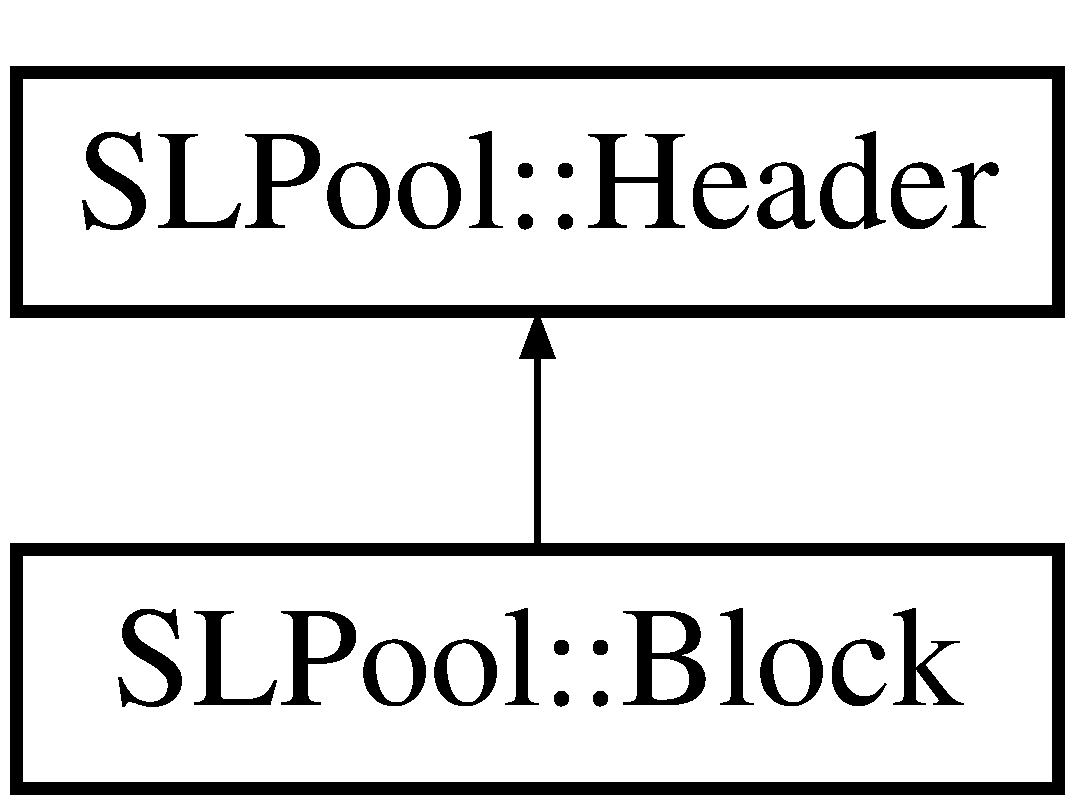
\includegraphics[height=2.000000cm]{struct_s_l_pool_1_1_block}
\end{center}
\end{figure}
\subsection*{Public Types}
\begin{DoxyCompactItemize}
\item 
enum \{ {\bfseries Block\+Size} = 16
 \}\hypertarget{struct_s_l_pool_1_1_block_adbb416e65dd0d7aa2121e30b34424db8}{}\label{struct_s_l_pool_1_1_block_adbb416e65dd0d7aa2121e30b34424db8}

\end{DoxyCompactItemize}
\subsection*{Public Attributes}
\begin{DoxyCompactItemize}
\item 
\begin{tabbing}
xx\=xx\=xx\=xx\=xx\=xx\=xx\=xx\=xx\=\kill
union \{\\
\>\hyperlink{struct_s_l_pool_1_1_block}{Block} $\ast$ {\bfseries mp\_Next}\\
\>char {\bfseries mc\_RawArea} \mbox{[}BlockSize-\/sizeof(\hyperlink{struct_s_l_pool_1_1_header}{Header})\mbox{]}\\
\}; \hypertarget{struct_s_l_pool_1_1_block_a77176c27d7b62721129f2d2539ec72b5}{}\label{struct_s_l_pool_1_1_block_a77176c27d7b62721129f2d2539ec72b5}
\\

\end{tabbing}\end{DoxyCompactItemize}


The documentation for this struct was generated from the following file\+:\begin{DoxyCompactItemize}
\item 
include/\hyperlink{slpool_8hpp}{slpool.\+hpp}\end{DoxyCompactItemize}

\hypertarget{class_event}{}\section{Event Class Reference}
\label{class_event}\index{Event@{Event}}


A class that creates a pair address/time-\/stamp.  




{\ttfamily \#include $<$event.\+hpp$>$}

\subsection*{Public Member Functions}
\begin{DoxyCompactItemize}
\item 
{\bfseries Event} (void $\ast$ptr, std\+::time\+\_\+t \+\_\+time)\hypertarget{class_event_a4c7bb7b8917287f04dbc38c4acdb1560}{}\label{class_event_a4c7bb7b8917287f04dbc38c4acdb1560}

\item 
std\+::time\+\_\+t {\bfseries get\+Time\+Stamp} ()\hypertarget{class_event_a10f30e1a322839fe772a6533d8681c4f}{}\label{class_event_a10f30e1a322839fe772a6533d8681c4f}

\item 
void $\ast$ {\bfseries get\+Memory\+Ptr} ()\hypertarget{class_event_ad251fb8313c6697932445d151c0fa0e2}{}\label{class_event_ad251fb8313c6697932445d151c0fa0e2}

\item 
bool {\bfseries operator$<$} (\hyperlink{class_event}{Event} m\+\_\+ptr2) const \hypertarget{class_event_afb9a087d9a508511b115cb5536160a76}{}\label{class_event_afb9a087d9a508511b115cb5536160a76}

\end{DoxyCompactItemize}


\subsection{Detailed Description}
A class that creates a pair address/time-\/stamp. 

The documentation for this class was generated from the following file\+:\begin{DoxyCompactItemize}
\item 
include/event.\+hpp\end{DoxyCompactItemize}

\hypertarget{struct_s_l_pool_1_1_header}{}\section{S\+L\+Pool\+:\+:Header Struct Reference}
\label{struct_s_l_pool_1_1_header}\index{S\+L\+Pool\+::\+Header@{S\+L\+Pool\+::\+Header}}
Inheritance diagram for S\+L\+Pool\+:\+:Header\+:\begin{figure}[H]
\begin{center}
\leavevmode
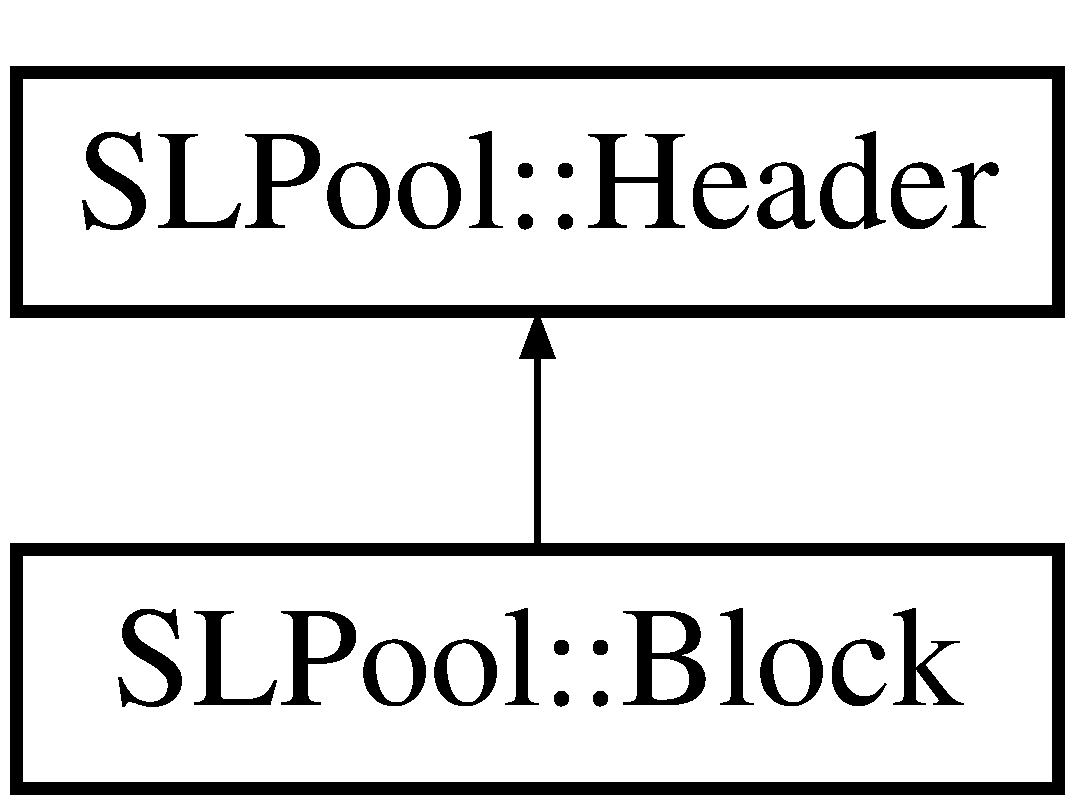
\includegraphics[height=2.000000cm]{struct_s_l_pool_1_1_header}
\end{center}
\end{figure}
\subsection*{Public Attributes}
\begin{DoxyCompactItemize}
\item 
unsigned int {\bfseries mui\+\_\+\+Length}\hypertarget{struct_s_l_pool_1_1_header_a0c06e96d58fa921e35411833364ad264}{}\label{struct_s_l_pool_1_1_header_a0c06e96d58fa921e35411833364ad264}

\end{DoxyCompactItemize}


The documentation for this struct was generated from the following file\+:\begin{DoxyCompactItemize}
\item 
include/\hyperlink{slpool_8hpp}{slpool.\+hpp}\end{DoxyCompactItemize}

\hypertarget{class_s_l_pool}{}\section{S\+L\+Pool Class Reference}
\label{class_s_l_pool}\index{S\+L\+Pool@{S\+L\+Pool}}
Inheritance diagram for S\+L\+Pool\+:\begin{figure}[H]
\begin{center}
\leavevmode
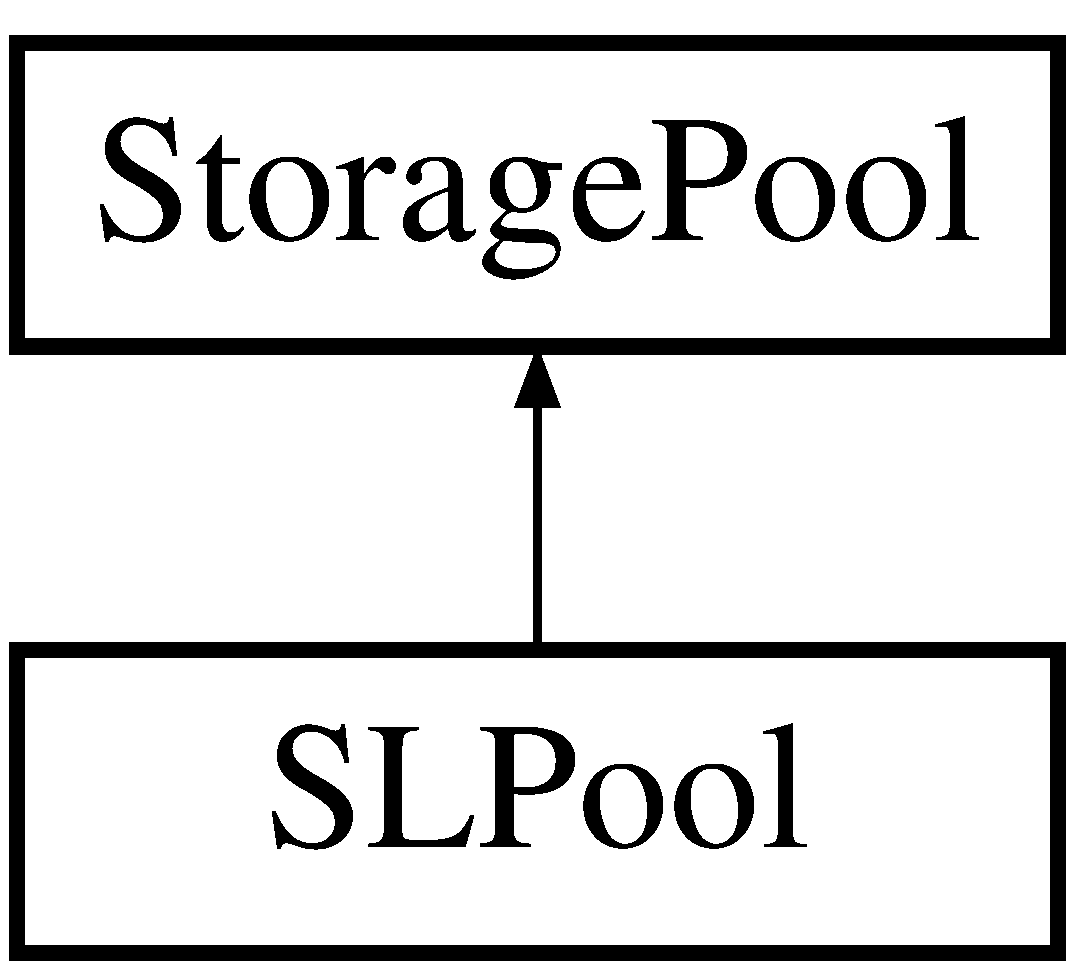
\includegraphics[height=2.000000cm]{class_s_l_pool}
\end{center}
\end{figure}
\subsection*{Classes}
\begin{DoxyCompactItemize}
\item 
struct \hyperlink{struct_s_l_pool_1_1_block}{Block}
\item 
struct \hyperlink{struct_s_l_pool_1_1_header}{Header}
\end{DoxyCompactItemize}
\subsection*{Public Member Functions}
\begin{DoxyCompactItemize}
\item 
{\bfseries S\+L\+Pool} (size\+\_\+type)\hypertarget{class_s_l_pool_a65f9984edead66802c8af56b0b32b3f8}{}\label{class_s_l_pool_a65f9984edead66802c8af56b0b32b3f8}

\item 
void $\ast$ \hyperlink{class_s_l_pool_a552b1b836f38cd997fb8d2471ed66383}{Allocate} (size\+\_\+type)
\begin{DoxyCompactList}\small\item\em This method reserve blocks in the pool according to the amount of bytes required. \end{DoxyCompactList}\item 
void $\ast$ \hyperlink{class_s_l_pool_a75bc0a6c01a3cd43959d56c339339baf}{Best\+\_\+\+Allocate} (size\+\_\+type)
\begin{DoxyCompactList}\small\item\em This method reserve blocks in the pool according to the amount of bytes required traing to find the best sapace to alloc. \end{DoxyCompactList}\item 
void \hyperlink{class_s_l_pool_aed31c75c4a2d56acd2f845dda2c5b1ad}{Free} (void $\ast$)
\begin{DoxyCompactList}\small\item\em This method frees the space on the pool. \end{DoxyCompactList}\item 
unsigned int \hyperlink{class_s_l_pool_a63cfa56c62750f1dd15a73d5a2ea42c3}{get\+Length} (size\+\_\+type)
\begin{DoxyCompactList}\small\item\em Calculate the number of blocks needed to a given amount of bytes. \end{DoxyCompactList}\item 
void \hyperlink{class_s_l_pool_a9085c8ec923b46f9f72eb1fed7637a6f}{view} ()
\begin{DoxyCompactList}\small\item\em Print the corrent state of the pool using \char`\"{}\mbox{[}\#\mbox{]}\char`\"{} to full space and \char`\"{}\mbox{[} \mbox{]}\char`\"{} to free space. \end{DoxyCompactList}\end{DoxyCompactItemize}


\subsection{Member Function Documentation}
\index{S\+L\+Pool@{S\+L\+Pool}!Allocate@{Allocate}}
\index{Allocate@{Allocate}!S\+L\+Pool@{S\+L\+Pool}}
\subsubsection[{\texorpdfstring{Allocate(size\+\_\+type)}{Allocate(size_type)}}]{\setlength{\rightskip}{0pt plus 5cm}void $\ast$ S\+L\+Pool\+::\+Allocate (
\begin{DoxyParamCaption}
\item[{size\+\_\+type}]{bytes}
\end{DoxyParamCaption}
)\hspace{0.3cm}{\ttfamily [virtual]}}\hypertarget{class_s_l_pool_a552b1b836f38cd997fb8d2471ed66383}{}\label{class_s_l_pool_a552b1b836f38cd997fb8d2471ed66383}


This method reserve blocks in the pool according to the amount of bytes required. 


\begin{DoxyParams}{Parameters}
{\em bytes} & The amount of bytes to reserve in the pool. \\
\hline
\end{DoxyParams}


Implements \hyperlink{class_storage_pool}{Storage\+Pool}.


\begin{DoxyCode}
30                                        \{
31     \textcolor{keywordtype}{bool} blockFound = \textcolor{keyword}{true};
32     Block *work = (&mr\_Sentinel)->mp\_Next;
33     Block *tail = &mr\_Sentinel;
34     size\_type length = \hyperlink{class_s_l_pool_a63cfa56c62750f1dd15a73d5a2ea42c3}{getLength}(bytes);
35 
36     \textcolor{keywordflow}{while}(work != \textcolor{keyword}{nullptr} and blockFound)\{\textcolor{comment}{// Run the whole SLPool.}
37         \textcolor{keywordflow}{if}(work->mui\_Length >= length)\{
38             \textcolor{keywordflow}{if}(work->mui\_Length == length)\{
39                 tail->mp\_Next = work->mp\_Next;
40             \}
41             \textcolor{keywordflow}{else}\{
42                 tail->mp\_Next = work+length;
43                 tail->mp\_Next->mp\_Next = work->mp\_Next;
44                 tail->mp\_Next->mui\_Length = work->mui\_Length-length;
45                 work->mui\_Length = length;
46             \}
47 
48             blockFound=\textcolor{keyword}{false};
49             \textcolor{keywordflow}{if}(mr\_Sentinel.mp\_Next == work)\textcolor{comment}{//Tail = actual block then skip one node}
50                 mr\_Sentinel.mp\_Next = work->mp\_Next;
51             \textcolor{keywordflow}{break};
52 
53         \} \textcolor{keywordflow}{else}\{
54             tail = tail->mp\_Next; \textcolor{comment}{// skip one node on last item}
55             work = work->mp\_Next; \textcolor{comment}{// skip one node on the actual node}
56         \}
57 
58         \textcolor{keywordflow}{if}(blockFound)
59             \textcolor{keywordflow}{throw} (std::bad\_alloc());
60     \}
61 
62     \textcolor{keywordflow}{return} \textcolor{keyword}{reinterpret\_cast<}\textcolor{keywordtype}{void} *\textcolor{keyword}{>}(\textcolor{keyword}{reinterpret\_cast<}Header *\textcolor{keyword}{>}(work)+1U);
63 \}
\end{DoxyCode}
\index{S\+L\+Pool@{S\+L\+Pool}!Best\+\_\+\+Allocate@{Best\+\_\+\+Allocate}}
\index{Best\+\_\+\+Allocate@{Best\+\_\+\+Allocate}!S\+L\+Pool@{S\+L\+Pool}}
\subsubsection[{\texorpdfstring{Best\+\_\+\+Allocate(size\+\_\+type)}{Best_Allocate(size_type)}}]{\setlength{\rightskip}{0pt plus 5cm}void $\ast$ S\+L\+Pool\+::\+Best\+\_\+\+Allocate (
\begin{DoxyParamCaption}
\item[{size\+\_\+type}]{bytes}
\end{DoxyParamCaption}
)}\hypertarget{class_s_l_pool_a75bc0a6c01a3cd43959d56c339339baf}{}\label{class_s_l_pool_a75bc0a6c01a3cd43959d56c339339baf}


This method reserve blocks in the pool according to the amount of bytes required traing to find the best sapace to alloc. 


\begin{DoxyParams}{Parameters}
{\em bytes} & The amount of bytes to reserve in the pool. \\
\hline
\end{DoxyParams}
$<$ Control if the allocation was already done. 
\begin{DoxyCode}
65                                              \{
66     \textcolor{keywordtype}{bool} blockAllocted = \textcolor{keyword}{false};
67     Block *work = (&mr\_Sentinel)->mp\_Next;
68     Block *best = \textcolor{keyword}{nullptr};\textcolor{comment}{// get the best free space for the allocation}
69     Block *tail = &mr\_Sentinel;
70     Block *tailaux = \textcolor{keyword}{nullptr};
71     size\_type length = \hyperlink{class_s_l_pool_a63cfa56c62750f1dd15a73d5a2ea42c3}{getLength}(bytes);
72 
73     \textcolor{keywordflow}{while}(work != \textcolor{keyword}{nullptr})\{\textcolor{comment}{// Run the whole SLPool.}
74         std::cout << &best << std::endl;
75         \textcolor{keywordflow}{if}(work->mui\_Length == length)\{\textcolor{comment}{// if the freespace is the sabe, allocate and finish.}
76             blockAllocted = \textcolor{keyword}{true};
77             tail->mp\_Next = work->mp\_Next;
78             \textcolor{keywordflow}{break};
79         \}
80         \textcolor{keywordflow}{else} \textcolor{keywordflow}{if}(best == \textcolor{keyword}{nullptr})\{
81             \textcolor{keywordflow}{if}(work->mui\_Length > length)\{
82                 best = work;
83                 tailaux = tail;
84             \}
85         \}
86         \textcolor{comment}{//look for the best option}
87         \textcolor{keywordflow}{else} \textcolor{keywordflow}{if}(work->mui\_Length > length and work->mui\_Length < best->mui\_Length)
88                 best = work;
89                 tailaux = tail;
90 
91         tail = tail->mp\_Next; \textcolor{comment}{// skip one node on last item}
92         work = work->mp\_Next; \textcolor{comment}{// skip one node on the actual node}
93     \}
94     \textcolor{keywordflow}{if}(!blockAllocted)\{
95         \textcolor{keywordflow}{if}( best == \textcolor{keyword}{nullptr}) \textcolor{comment}{//If it don't found any possible position: erro bad\_alloc}
96             \textcolor{keywordflow}{throw} (std::bad\_alloc());
97         \textcolor{keywordflow}{else}\{ \textcolor{comment}{// allocate in the best option}
98             tailaux->mp\_Next = best+length;
99             tailaux->mp\_Next->mp\_Next = best->mp\_Next;
100             tailaux->mp\_Next->mui\_Length = best->mui\_Length-length;
101             best->mui\_Length = length;
102         \}
103     \}
104     \textcolor{keywordflow}{return} \textcolor{keyword}{reinterpret\_cast<}\textcolor{keywordtype}{void} *\textcolor{keyword}{>}(\textcolor{keyword}{reinterpret\_cast<}Header *\textcolor{keyword}{>}(best)+1U);
105 \}
\end{DoxyCode}
\index{S\+L\+Pool@{S\+L\+Pool}!Free@{Free}}
\index{Free@{Free}!S\+L\+Pool@{S\+L\+Pool}}
\subsubsection[{\texorpdfstring{Free(void $\ast$)}{Free(void *)}}]{\setlength{\rightskip}{0pt plus 5cm}void S\+L\+Pool\+::\+Free (
\begin{DoxyParamCaption}
\item[{void $\ast$}]{pt\+Reserved}
\end{DoxyParamCaption}
)\hspace{0.3cm}{\ttfamily [virtual]}}\hypertarget{class_s_l_pool_aed31c75c4a2d56acd2f845dda2c5b1ad}{}\label{class_s_l_pool_aed31c75c4a2d56acd2f845dda2c5b1ad}


This method frees the space on the pool. 


\begin{DoxyParams}{Parameters}
{\em pt\+Reserved} & A pointer to the space that what to free. \\
\hline
\end{DoxyParams}


Implements \hyperlink{class_storage_pool}{Storage\+Pool}.


\begin{DoxyCode}
107                                    \{
108     Block* ptPostReserved = mr\_Sentinel.mp\_Next;
109     Block* ptPrevReserved = &mr\_Sentinel;
110     Block* reserveBlock = reinterpret\_cast <Block*>(reinterpret\_cast <\textcolor{keywordtype}{int}*>(ptReserved)-1U);;
111 
112     \textcolor{keywordflow}{while}(ptPostReserved != \textcolor{keyword}{nullptr})\{
113         \textcolor{keywordflow}{if}(ptPostReserved > reserveBlock)\{
114             \textcolor{keywordflow}{if}(((ptPrevReserved+ptPrevReserved->mui\_Length) == reserveBlock ) && ((reserveBlock+
      reserveBlock->mui\_Length) == ptPostReserved))\{
115                 ptPrevReserved->mp\_Next = ptPostReserved->mp\_Next; \textcolor{comment}{// Prev areas freed}
116                 ptPrevReserved->mui\_Length += reserveBlock->mui\_Length+ptPostReserved->mui\_Length; \textcolor{comment}{//
       Combine all 3 areas in one node}
117                 reserveBlock->mui\_Length = 0; \textcolor{comment}{// reset reserve pointer}
118                 ptPostReserved->mui\_Length = 0; \textcolor{comment}{// reset post pointer}
119             \} \textcolor{keywordflow}{else} \textcolor{keywordflow}{if} ((ptPrevReserved+ptPrevReserved->mui\_Length) == reserveBlock)\{ \textcolor{comment}{// sum of the areas is
       the same of the reserved block that will be liberated}
120                 \textcolor{comment}{//TODO: Combine the reserved area with the prev; reset prev area; point the reserved area
       to the prev.}
121                 ptPrevReserved->mp\_Next = ptPostReserved->mp\_Next; \textcolor{comment}{// Prev areas freed}
122                 ptPrevReserved->mui\_Length += reserveBlock->mui\_Length;
123                 reserveBlock->mui\_Length = 0; \textcolor{comment}{// reset reserve pointer}
124             \} \textcolor{keywordflow}{else} \textcolor{keywordflow}{if} ((reserveBlock+reserveBlock->mui\_Length) == ptPostReserved)\{ \textcolor{comment}{// sum of the reserved
       block are the same of the post pointer}
125                 \textcolor{comment}{//TODO:}
126                 reserveBlock->mp\_Next = ptPostReserved->mp\_Next; \textcolor{comment}{// Prev areas freed}
127                 ptPrevReserved->mp\_Next=reserveBlock;
128                 reserveBlock->mui\_Length += ptPostReserved->mui\_Length;
129                 ptPostReserved->mui\_Length = 0; \textcolor{comment}{// reset reserve pointer}
130             \} \textcolor{keywordflow}{else}\{
131                 \textcolor{comment}{//TODO: The prev area must be freed and the post is reserved. Free the are and sum with the
       prev.}
132                 ptPrevReserved->mp\_Next = reserveBlock;
133                 reserveBlock->mp\_Next = ptPostReserved;
134             \}
135             reserveBlock = \textcolor{keyword}{nullptr};
136             \textcolor{keywordflow}{break};
137         \}\textcolor{keywordflow}{else}\{
138             ptPrevReserved=ptPrevReserved->mp\_Next;
139         \}
140         ptPostReserved=ptPostReserved->mp\_Next;
141     \}
142 
143     \textcolor{keywordflow}{if}(ptPostReserved == \textcolor{keyword}{nullptr})\{
144         reserveBlock->mp\_Next=ptPostReserved;
145         ptPrevReserved->mp\_Next=reserveBlock;
146         reserveBlock->mp\_Next = \textcolor{keyword}{nullptr};
147 
148     \}
149 \}
\end{DoxyCode}
\index{S\+L\+Pool@{S\+L\+Pool}!get\+Length@{get\+Length}}
\index{get\+Length@{get\+Length}!S\+L\+Pool@{S\+L\+Pool}}
\subsubsection[{\texorpdfstring{get\+Length(size\+\_\+type)}{getLength(size_type)}}]{\setlength{\rightskip}{0pt plus 5cm}unsigned int S\+L\+Pool\+::get\+Length (
\begin{DoxyParamCaption}
\item[{size\+\_\+type}]{bytes}
\end{DoxyParamCaption}
)}\hypertarget{class_s_l_pool_a63cfa56c62750f1dd15a73d5a2ea42c3}{}\label{class_s_l_pool_a63cfa56c62750f1dd15a73d5a2ea42c3}


Calculate the number of blocks needed to a given amount of bytes. 


\begin{DoxyParams}{Parameters}
{\em Bytes} & number of bytes to be allocated \\
\hline
\end{DoxyParams}
\begin{DoxyReturn}{Returns}
The amount of blocks needed. 
\end{DoxyReturn}

\begin{DoxyCode}
151                                              \{
152     \textcolor{keywordtype}{int} tst = std::ceil(static\_cast<float>(bytes)/Block::BlockSize); 
153     \textcolor{keywordflow}{return} tst;
154 \}
\end{DoxyCode}
\index{S\+L\+Pool@{S\+L\+Pool}!view@{view}}
\index{view@{view}!S\+L\+Pool@{S\+L\+Pool}}
\subsubsection[{\texorpdfstring{view()}{view()}}]{\setlength{\rightskip}{0pt plus 5cm}void S\+L\+Pool\+::view (
\begin{DoxyParamCaption}
{}
\end{DoxyParamCaption}
)\hspace{0.3cm}{\ttfamily [virtual]}}\hypertarget{class_s_l_pool_a9085c8ec923b46f9f72eb1fed7637a6f}{}\label{class_s_l_pool_a9085c8ec923b46f9f72eb1fed7637a6f}


Print the corrent state of the pool using \char`\"{}\mbox{[}\#\mbox{]}\char`\"{} to full space and \char`\"{}\mbox{[} \mbox{]}\char`\"{} to free space. 

$<$ Gets the number of block in the Pool

$<$ Used to get the number of blocks occupied by the free/full space

$<$ A pointer to the next free space in the pool 

Implements \hyperlink{class_storage_pool}{Storage\+Pool}.


\begin{DoxyCode}
156                  \{
157       \textcolor{keywordtype}{int} total\_length = mui\_NumberOfBlocks; 
158     \textcolor{keywordtype}{int} length; 
159     \textcolor{keywordtype}{int} free\_length = 0;
160     \textcolor{keywordtype}{int} full\_length = 0;
161     Block* next\_free = (&mr\_Sentinel)->mp\_Next; 
162 
163     std::cout << \textcolor{stringliteral}{"| "};
164     \textcolor{keywordflow}{for} (\textcolor{keyword}{auto} i = 0; i < total\_length; i += length) \{
165         length = mp\_Pool[i].mui\_Length;
166         \textcolor{keywordflow}{if}(&mp\_Pool[i] == next\_free)\{ \textcolor{comment}{// If is a free space and print [#] to each block}
167             \textcolor{keywordflow}{for} (\textcolor{keyword}{auto} e = 0; e < length; e++) \{
168                     std::cout << \textcolor{stringliteral}{"[ ]"};
169             \}
170             std::cout << \textcolor{stringliteral}{" | "};
171             free\_length += length;
172             next\_free = mp\_Pool[i].mp\_Next;
173         \}
174         \textcolor{keywordflow}{else} \{\textcolor{comment}{// Else, if is the space is full and print [#] to each block}
175             \textcolor{keywordflow}{for} (\textcolor{keyword}{auto} e = 0; e < length; e++) \{
176                 std::cout << \textcolor{stringliteral}{"[#]"};
177             \}
178             std::cout << \textcolor{stringliteral}{" | "};
179             full\_length += length;
180         \}
181     \}
182      std::cout << \textcolor{stringliteral}{"\(\backslash\)n\(\backslash\)n\(\backslash\)t>>> Number of free blocks: "} << free\_length << std::endl;
183      std::cout << \textcolor{stringliteral}{"\(\backslash\)t>>> Number of allocated blocks: "} << full\_length << \textcolor{stringliteral}{"\(\backslash\)n"} << std::endl;
184 \}
\end{DoxyCode}


The documentation for this class was generated from the following files\+:\begin{DoxyCompactItemize}
\item 
include/\hyperlink{slpool_8hpp}{slpool.\+hpp}\item 
include/\hyperlink{slpool_8inl}{slpool.\+inl}\end{DoxyCompactItemize}

\hypertarget{class_storage_pool}{}\section{Storage\+Pool Class Reference}
\label{class_storage_pool}\index{Storage\+Pool@{Storage\+Pool}}
Inheritance diagram for Storage\+Pool\+:\begin{figure}[H]
\begin{center}
\leavevmode
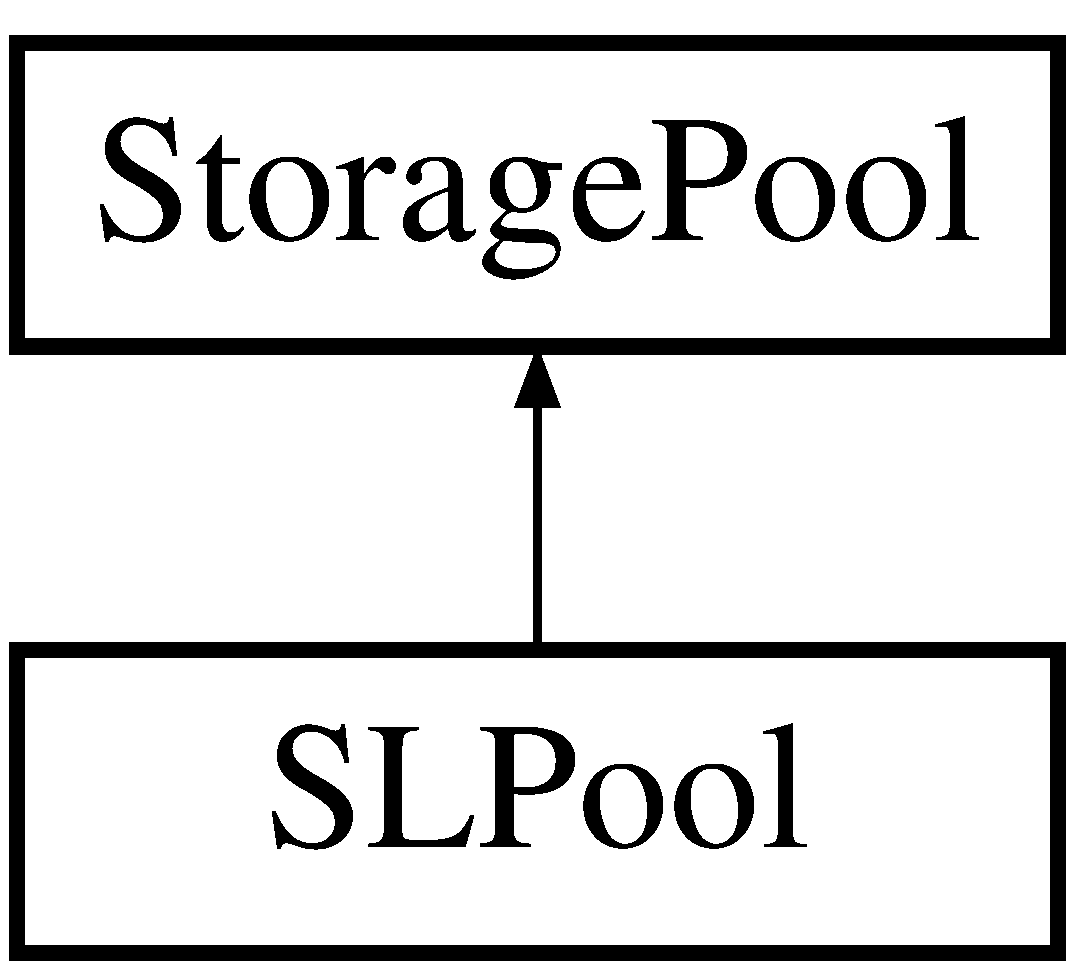
\includegraphics[height=2.000000cm]{class_storage_pool}
\end{center}
\end{figure}
\subsection*{Public Member Functions}
\begin{DoxyCompactItemize}
\item 
virtual void $\ast$ {\bfseries Allocate} (std\+::size\+\_\+t)=0\hypertarget{class_storage_pool_a41c66733db91a537c883c939996723b7}{}\label{class_storage_pool_a41c66733db91a537c883c939996723b7}

\item 
virtual void {\bfseries Free} (void $\ast$)=0\hypertarget{class_storage_pool_a2120a75c4562735372d089685828b8df}{}\label{class_storage_pool_a2120a75c4562735372d089685828b8df}

\item 
virtual void {\bfseries view} ()=0\hypertarget{class_storage_pool_a5e5484141dce4e835bed1153b1f0b662}{}\label{class_storage_pool_a5e5484141dce4e835bed1153b1f0b662}

\end{DoxyCompactItemize}


The documentation for this class was generated from the following file\+:\begin{DoxyCompactItemize}
\item 
include/storagepool.\+hpp\end{DoxyCompactItemize}

\hypertarget{struct_tag}{}\section{Tag Struct Reference}
\label{struct_tag}\index{Tag@{Tag}}
\subsection*{Public Attributes}
\begin{DoxyCompactItemize}
\item 
\hyperlink{class_storage_pool}{Storage\+Pool} $\ast$ {\bfseries pool}\hypertarget{struct_tag_aa4adbc74180401c6e0bff0a4c429f37e}{}\label{struct_tag_aa4adbc74180401c6e0bff0a4c429f37e}

\end{DoxyCompactItemize}


The documentation for this struct was generated from the following file\+:\begin{DoxyCompactItemize}
\item 
include/allocate.\+hpp\end{DoxyCompactItemize}

\chapter{File Documentation}
\hypertarget{allocate_8inl}{}\section{include/allocate.inl File Reference}
\label{allocate_8inl}\index{include/allocate.\+inl@{include/allocate.\+inl}}


G\+R\+E\+M\+L\+I\+NS Implementation.  


{\ttfamily \#include \char`\"{}storagepool.\+hpp\char`\"{}}\\*
\subsection*{Functions}
\begin{DoxyCompactItemize}
\item 
void $\ast$ {\bfseries operator new} (size\+\_\+type bytes, \hyperlink{class_storage_pool}{Storage\+Pool} \&p)\hypertarget{allocate_8inl_af955c2484913d10f828dd418b7c8ebeb}{}\label{allocate_8inl_af955c2484913d10f828dd418b7c8ebeb}

\item 
void $\ast$ {\bfseries operator new} (size\+\_\+type bytes)\hypertarget{allocate_8inl_aa886d6c22d8dd32cccaf0a2fc2aea2a2}{}\label{allocate_8inl_aa886d6c22d8dd32cccaf0a2fc2aea2a2}

\item 
void {\bfseries operator delete} (void $\ast$arg) noexcept\hypertarget{allocate_8inl_a49aeafb236d8e2fa3f1b687b6e0122db}{}\label{allocate_8inl_a49aeafb236d8e2fa3f1b687b6e0122db}

\end{DoxyCompactItemize}


\subsection{Detailed Description}
G\+R\+E\+M\+L\+I\+NS Implementation. 

\begin{DoxyAuthor}{Author}
Johnnylee Bryan Marques da Rocha e Pedro Arthur Medeiros Fernandes. 
\end{DoxyAuthor}
\begin{DoxyCopyright}{Copyright}
Copyright \copyright{} 2016. All rights reserved.
\end{DoxyCopyright}
File with the implementations of new operators. 
\hypertarget{slpool_8hpp}{}\section{include/slpool.hpp File Reference}
\label{slpool_8hpp}\index{include/slpool.\+hpp@{include/slpool.\+hpp}}


G\+R\+E\+M\+L\+I\+NS Implementation.  


{\ttfamily \#include $<$iostream$>$}\\*
{\ttfamily \#include \char`\"{}storagepool.\+hpp\char`\"{}}\\*
{\ttfamily \#include \char`\"{}slpool.\+inl\char`\"{}}\\*
\subsection*{Classes}
\begin{DoxyCompactItemize}
\item 
class \hyperlink{class_s_l_pool}{S\+L\+Pool}
\item 
struct \hyperlink{struct_s_l_pool_1_1_header}{S\+L\+Pool\+::\+Header}
\item 
struct \hyperlink{struct_s_l_pool_1_1_block}{S\+L\+Pool\+::\+Block}
\end{DoxyCompactItemize}
\subsection*{Typedefs}
\begin{DoxyCompactItemize}
\item 
typedef std\+::size\+\_\+t {\bfseries size\+\_\+type}\hypertarget{slpool_8hpp_a89a6dcafb6130e3e1bcd6d1285e0dd6f}{}\label{slpool_8hpp_a89a6dcafb6130e3e1bcd6d1285e0dd6f}

\end{DoxyCompactItemize}


\subsection{Detailed Description}
G\+R\+E\+M\+L\+I\+NS Implementation. 

\begin{DoxyAuthor}{Author}
Johnnylee Bryan Marques da Rocha e Pedro Arthur Medeiros Fernandes. 
\end{DoxyAuthor}
\begin{DoxyCopyright}{Copyright}
Copyright \copyright{} 2016. All rights reserved.
\end{DoxyCopyright}
File with the declaration of the class \hyperlink{class_s_l_pool}{S\+L\+Pool} used to modfy the memory.

\begin{DoxyAuthor}{Author}
Johnnylee Bryan Marques da Rocha e Pedro Arthur Medeiros Fernandes. 
\end{DoxyAuthor}
\begin{DoxyCopyright}{Copyright}
Copyright \copyright{} 2016. All rights reserved.
\end{DoxyCopyright}
File with the declaration of the class Storege\+Pool that have the main functions. 
\hypertarget{slpool_8inl}{}\section{include/slpool.inl File Reference}
\label{slpool_8inl}\index{include/slpool.\+inl@{include/slpool.\+inl}}


G\+R\+E\+M\+L\+I\+NS Implementation.  


{\ttfamily \#include $<$iostream$>$}\\*
{\ttfamily \#include $<$cmath$>$}\\*
{\ttfamily \#include $<$new$>$}\\*
{\ttfamily \#include \char`\"{}allocate.\+hpp\char`\"{}}\\*
{\ttfamily \#include \char`\"{}storagepool.\+hpp\char`\"{}}\\*
\subsection*{Typedefs}
\begin{DoxyCompactItemize}
\item 
typedef std\+::size\+\_\+t {\bfseries size\+\_\+type}\hypertarget{slpool_8inl_a89a6dcafb6130e3e1bcd6d1285e0dd6f}{}\label{slpool_8inl_a89a6dcafb6130e3e1bcd6d1285e0dd6f}

\end{DoxyCompactItemize}


\subsection{Detailed Description}
G\+R\+E\+M\+L\+I\+NS Implementation. 

\begin{DoxyAuthor}{Author}
Johnnylee Bryan Marques da Rocha e Pedro Arthur Medeiros Fernandes. 
\end{DoxyAuthor}
\begin{DoxyCopyright}{Copyright}
Copyright \copyright{} 2016. All rights reserved.
\end{DoxyCopyright}
File with the implementatio of the class \hyperlink{class_s_l_pool}{S\+L\+Pool} used to modfy the memory. 
\hypertarget{drive__gremlins_8cpp}{}\section{src/drive\+\_\+gremlins.cpp File Reference}
\label{drive__gremlins_8cpp}\index{src/drive\+\_\+gremlins.\+cpp@{src/drive\+\_\+gremlins.\+cpp}}


G\+R\+E\+M\+L\+I\+NS Implementation.  


{\ttfamily \#include $<$iostream$>$}\\*
{\ttfamily \#include $<$ctime$>$}\\*
{\ttfamily \#include $<$cstdlib$>$}\\*
{\ttfamily \#include $<$queue$>$}\\*
{\ttfamily \#include $<$chrono$>$}\\*
{\ttfamily \#include \char`\"{}allocate.\+hpp\char`\"{}}\\*
{\ttfamily \#include \char`\"{}slpool.\+hpp\char`\"{}}\\*
{\ttfamily \#include \char`\"{}event.\+hpp\char`\"{}}\\*
\subsection*{Functions}
\begin{DoxyCompactItemize}
\item 
std\+::time\+\_\+t \hyperlink{drive__gremlins_8cpp_a21e7c7c79ca75da72264d748ba0d481d}{get\+Random\+Time\+Interval} ()
\begin{DoxyCompactList}\small\item\em Setup random numbers generator for memory size , say \mbox{[}100, 2000\mbox{]} bytes. \end{DoxyCompactList}\item 
int \hyperlink{drive__gremlins_8cpp_a0aa6261ed80350fb37777559d4fed2a1}{get\+Random\+For\+Size} ()
\begin{DoxyCompactList}\small\item\em Setup random numbers generator for time intervals , say \mbox{[}1, 100\mbox{]} units. \end{DoxyCompactList}\item 
void \hyperlink{drive__gremlins_8cpp_a370ac5b02ea1189b139175e030cb9716}{Storage\+Pool\+Test} (\hyperlink{class_storage_pool}{Storage\+Pool} \&\+\_\+pool, std\+::time\+\_\+t \+\_\+time\+Limit)
\begin{DoxyCompactList}\small\item\em test the alocation of memory using the \hyperlink{class_storage_pool}{Storage\+Pool} \end{DoxyCompactList}\item 
void \hyperlink{drive__gremlins_8cpp_a64b701d8f9dd3687aaa00af6e8becb23}{S\+O\+Memory\+Test} (std\+::time\+\_\+t \+\_\+time\+Limit)
\begin{DoxyCompactList}\small\item\em Test the alocation of memory using the OS methods. \end{DoxyCompactList}\item 
int {\bfseries main} (int argc, char const $\ast$argv\mbox{[}$\,$\mbox{]})\hypertarget{drive__gremlins_8cpp_abf9e6b7e6f15df4b525a2e7705ba3089}{}\label{drive__gremlins_8cpp_abf9e6b7e6f15df4b525a2e7705ba3089}

\end{DoxyCompactItemize}


\subsection{Detailed Description}
G\+R\+E\+M\+L\+I\+NS Implementation. 

\begin{DoxyAuthor}{Author}
Johnnylee Bryan Marques da Rocha e Pedro Arthur Medeiros Fernandes. 
\end{DoxyAuthor}
\begin{DoxyCopyright}{Copyright}
Copyright \copyright{} 2016. All rights reserved.
\end{DoxyCopyright}
File with a tast comparing the G\+R\+E\+M\+L\+I\+NS implementation with the OS.

\begin{DoxyAuthor}{Author}
Johnnylee Bryan Marques da Rocha e Pedro Arthur Medeiros Fernandes. 
\end{DoxyAuthor}
\begin{DoxyCopyright}{Copyright}
Copyright \copyright{} 2016. All rights reserved.
\end{DoxyCopyright}
File with a tast to pruve that the class \hyperlink{class_s_l_pool}{S\+L\+Pool} is working. 

\subsection{Function Documentation}
\index{drive\+\_\+gremlins.\+cpp@{drive\+\_\+gremlins.\+cpp}!get\+Random\+For\+Size@{get\+Random\+For\+Size}}
\index{get\+Random\+For\+Size@{get\+Random\+For\+Size}!drive\+\_\+gremlins.\+cpp@{drive\+\_\+gremlins.\+cpp}}
\subsubsection[{\texorpdfstring{get\+Random\+For\+Size()}{getRandomForSize()}}]{\setlength{\rightskip}{0pt plus 5cm}int get\+Random\+For\+Size (
\begin{DoxyParamCaption}
{}
\end{DoxyParamCaption}
)}\hypertarget{drive__gremlins_8cpp_a0aa6261ed80350fb37777559d4fed2a1}{}\label{drive__gremlins_8cpp_a0aa6261ed80350fb37777559d4fed2a1}


Setup random numbers generator for time intervals , say \mbox{[}1, 100\mbox{]} units. 

\begin{DoxyReturn}{Returns}
A random number in the range \mbox{[}1, 100\mbox{]}. 
\end{DoxyReturn}

\begin{DoxyCode}
34                       \{
35     \textcolor{keywordflow}{return} 100 + (rand() % 2000 - 100);
36 \}
\end{DoxyCode}
\index{drive\+\_\+gremlins.\+cpp@{drive\+\_\+gremlins.\+cpp}!get\+Random\+Time\+Interval@{get\+Random\+Time\+Interval}}
\index{get\+Random\+Time\+Interval@{get\+Random\+Time\+Interval}!drive\+\_\+gremlins.\+cpp@{drive\+\_\+gremlins.\+cpp}}
\subsubsection[{\texorpdfstring{get\+Random\+Time\+Interval()}{getRandomTimeInterval()}}]{\setlength{\rightskip}{0pt plus 5cm}std\+::time\+\_\+t get\+Random\+Time\+Interval (
\begin{DoxyParamCaption}
{}
\end{DoxyParamCaption}
)}\hypertarget{drive__gremlins_8cpp_a21e7c7c79ca75da72264d748ba0d481d}{}\label{drive__gremlins_8cpp_a21e7c7c79ca75da72264d748ba0d481d}


Setup random numbers generator for memory size , say \mbox{[}100, 2000\mbox{]} bytes. 

\begin{DoxyReturn}{Returns}
A random number in the range \mbox{[}100, 2000\mbox{]}. 
\end{DoxyReturn}

\begin{DoxyCode}
26                                  \{
27     \textcolor{keywordflow}{return} 1 + (rand() % 100 - 1);
28 \}
\end{DoxyCode}
\index{drive\+\_\+gremlins.\+cpp@{drive\+\_\+gremlins.\+cpp}!S\+O\+Memory\+Test@{S\+O\+Memory\+Test}}
\index{S\+O\+Memory\+Test@{S\+O\+Memory\+Test}!drive\+\_\+gremlins.\+cpp@{drive\+\_\+gremlins.\+cpp}}
\subsubsection[{\texorpdfstring{S\+O\+Memory\+Test(std\+::time\+\_\+t \+\_\+time\+Limit)}{SOMemoryTest(std::time_t _timeLimit)}}]{\setlength{\rightskip}{0pt plus 5cm}void S\+O\+Memory\+Test (
\begin{DoxyParamCaption}
\item[{std\+::time\+\_\+t}]{\+\_\+time\+Limit}
\end{DoxyParamCaption}
)}\hypertarget{drive__gremlins_8cpp_a64b701d8f9dd3687aaa00af6e8becb23}{}\label{drive__gremlins_8cpp_a64b701d8f9dd3687aaa00af6e8becb23}


Test the alocation of memory using the OS methods. 


\begin{DoxyParams}{Parameters}
{\em \+\_\+time\+Limit} & The limit time a block can be allocated. \\
\hline
\end{DoxyParams}

\begin{DoxyCode}
69                                         \{
70     std::priority\_queue<Event> pq;
71     
72     \textcolor{keywordflow}{for}( std::time\_t t (0); t < \_timeLimit; ++t )\{
73         \textcolor{keywordflow}{while}(!pq.empty()) \{ \textcolor{comment}{// Run while we have events pending or time to run .}
74             \hyperlink{class_event}{Event} ev = pq.top(); \textcolor{comment}{// Access the event with the smallest time - stamp .}
75             \textcolor{keywordflow}{if}(ev.getTimeStamp() > t) \textcolor{keywordflow}{break} ; \textcolor{comment}{// Still some time left ....}
76             
77             \textcolor{comment}{// When we got here , the top event has run out of time .}
78             pq.pop(); \textcolor{comment}{// Remove event from priority queue .}
79             std::free(ev.getMemoryPtr()); \textcolor{comment}{// Calling free operator .}
80         \}
81     \textcolor{keyword}{auto} memSize = \hyperlink{drive__gremlins_8cpp_a0aa6261ed80350fb37777559d4fed2a1}{getRandomForSize} ();
82     \textcolor{keywordtype}{void} * \textcolor{keyword}{const} add = std::malloc(memSize);
83     \textcolor{keyword}{auto} elapsedTime = \hyperlink{drive__gremlins_8cpp_a21e7c7c79ca75da72264d748ba0d481d}{getRandomTimeInterval}();
84     std::time\_t releaseTime = t+elapsedTime ; \textcolor{comment}{// Set time stamp some time from now .}
85     pq.push(\hyperlink{class_event}{Event} (add, releaseTime)); \textcolor{comment}{// Creating a new simulation event .}
86     \}
87 \}
\end{DoxyCode}
\index{drive\+\_\+gremlins.\+cpp@{drive\+\_\+gremlins.\+cpp}!Storage\+Pool\+Test@{Storage\+Pool\+Test}}
\index{Storage\+Pool\+Test@{Storage\+Pool\+Test}!drive\+\_\+gremlins.\+cpp@{drive\+\_\+gremlins.\+cpp}}
\subsubsection[{\texorpdfstring{Storage\+Pool\+Test(\+Storage\+Pool \&\+\_\+pool, std\+::time\+\_\+t \+\_\+time\+Limit)}{StoragePoolTest(StoragePool &_pool, std::time_t _timeLimit)}}]{\setlength{\rightskip}{0pt plus 5cm}void Storage\+Pool\+Test (
\begin{DoxyParamCaption}
\item[{{\bf Storage\+Pool} \&}]{\+\_\+pool, }
\item[{std\+::time\+\_\+t}]{\+\_\+time\+Limit}
\end{DoxyParamCaption}
)}\hypertarget{drive__gremlins_8cpp_a370ac5b02ea1189b139175e030cb9716}{}\label{drive__gremlins_8cpp_a370ac5b02ea1189b139175e030cb9716}


test the alocation of memory using the \hyperlink{class_storage_pool}{Storage\+Pool} 


\begin{DoxyParams}{Parameters}
{\em \+\_\+pool} & The \hyperlink{class_s_l_pool}{S\+L\+Pool} criated where the thins will be allocated. \\
\hline
{\em \+\_\+time\+Limit} & The Max time a block can be allocated; \\
\hline
\end{DoxyParams}

\begin{DoxyCode}
44                                                                  \{
45     std::priority\_queue<Event> pq;
46     
47     \textcolor{keywordflow}{for}( std::time\_t t (0); t < \_timeLimit; ++t )\{
48         \textcolor{keywordflow}{while}(!pq.empty()) \{ \textcolor{comment}{// Run while we have events pending or time to run .}
49             \hyperlink{class_event}{Event} ev = pq.top(); \textcolor{comment}{// Access the event with the smallest time - stamp .}
50             \textcolor{keywordflow}{if}(ev.getTimeStamp() > t) \textcolor{keywordflow}{break} ; \textcolor{comment}{// Still some time left ....}
51             
52             \textcolor{comment}{// When we got here , the top event has run out of time .}
53             pq.pop(); \textcolor{comment}{// Remove event from priority queue .}
54             \_pool.Free(ev.getMemoryPtr()); \textcolor{comment}{// Calling free operator .}
55         \}
56     \textcolor{keyword}{auto} memSize = \hyperlink{drive__gremlins_8cpp_a0aa6261ed80350fb37777559d4fed2a1}{getRandomForSize} ();
57     \textcolor{keywordtype}{void} * \textcolor{keyword}{const} add = \_pool.Allocate(memSize);
58     \textcolor{keyword}{auto} elapsedTime = \hyperlink{drive__gremlins_8cpp_a21e7c7c79ca75da72264d748ba0d481d}{getRandomTimeInterval}();
59     std::time\_t releaseTime = t+elapsedTime ; \textcolor{comment}{// Set time stamp some time from now .}
60     pq.push(\hyperlink{class_event}{Event}(add, releaseTime)); \textcolor{comment}{// Creating a new simulation event .}
61     \}
62 \}
\end{DoxyCode}

%--- End generated contents ---

% Index
\backmatter
\newpage
\phantomsection
\clearemptydoublepage
\addcontentsline{toc}{chapter}{Index}
\printindex

\end{document}
